\documentclass{beamer}

\beamertemplatenavigationsymbolsempty

\title{Polyhedral design\\with blended $n$-sided interpolants}
\author{P\'eter Salvi}
\institute{Budapest University of Technology and Economics}
\date{GrafGeo'24\\\vspace{1em}Budapest, April 10--11, 2024}

\begin{document}

\begin{frame}
  \titlepage
\end{frame}

\begin{frame}
  \frametitle{Outline}
  \begin{columns}
    \column{0.5\textwidth}
    \tableofcontents
    \column{0.5\textwidth}
    \centering
    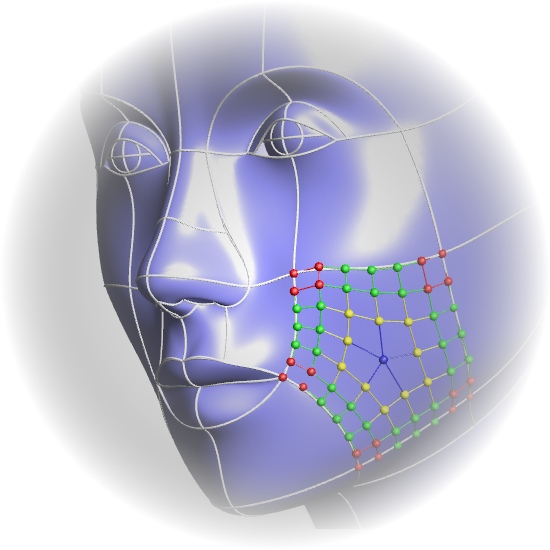
\includegraphics[width=\textwidth]{images/face-gradient.png}\\\vspace{1em}
  \end{columns}
  \centering
  
\includegraphics[height=2.5em]{images/iit.png}$\qquad$
  
\includegraphics[height=3em]{images/bme.jpg}
\end{frame}

\section{Motivation}

\end{document}
